% write your main thesis in logical individual chapters
% for better organization use a separate folder for images 
\graphicspath{{img/}}









%==============================
\chapter{Chapter X}
\label{chap:x}


%-----
\section{intro section}
Use figures like \ref{fig:x} to make your ideas more comprehensible. Figure captions should be descriptive. A reader should understand what is being displayed just by reading the caption, not needing to delve into the main body of the text. For any thing that has not been done by you provide adequate acknowledgement either by referencing the scientific work \cite{adami:1998, bentley:2002, reynolds:1978, reynolds:1987, lebar_bajec:2005a, lebar_bajec:2005b, heppner:1990} or through the Acknowledgements chapter. The Internet and Google can serve as good starting points for writing a thesis, especially since there can be found many tutorials.\footnote{\href{http://www.phys.unsw.edu.au/~jw/thesis.html}{http://www.phys.unsw.edu.au/\textasciitilde jw/thesis.html}}

\begin{figure}
 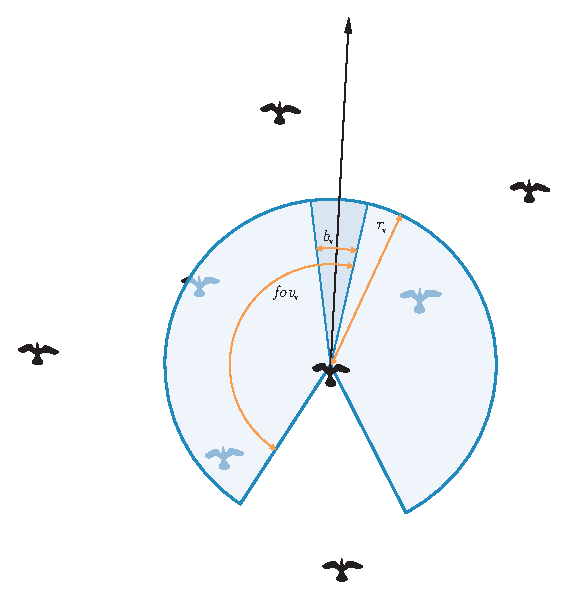
\includegraphics{fig[perception]}
 \caption{The perception model used in the fuzzy animat. The black arrow represents the fuzzy digital bird's flight direction. The shaded area represents the visual volume defined by the visual range $r_\mathrm{v}$, per eye visual field $f\kern-1.5ptov_\mathrm{v}$ and the angle of binocular overlap $b_\mathrm{v}$. The perceived flockmates are depicted in a light blue colour.}
 \label{fig:x}
\end{figure}


%-----
\section{...}
